\documentclass{beamer}
\usetheme[block = fill, titleformat title = allcaps, titleformat subtitle  = smallcaps, background = light]{metropolis}           % Use metropolis theme
\usetikzlibrary{arrows.meta,positioning}
\title{Housing market and migration revisited}
\subtitle{A multilevel gravity model for Dutch municipalities}
\date{\today}
\author{Thomas de Graaff}
\institute{Vrije Universiteit Amsterdam\\Department of Spatial Economics}
\begin{document}
\maketitle

\section{The problem}

  \begin{frame}{Background}
    	\begin{itemize}
    		\item 50--70\% of all research questions in spatial economics evolve around policy \alert{evaluation} 
    		\begin{itemize}
    			\item focus on \textbf{consistency}
    		\end{itemize}
    		\item Huge demand (e.g., by firms \& government) for research dealing with \alert{prediction}
    		\begin{itemize}
    			\item focus on model \textbf{performance}
    		\end{itemize}
    		\item But, more than 90\% of all statistical analyses is basic applied econometrics using \alert{linear} models and \alert{fixed} effects
    	\end{itemize}
  \end{frame}

\begin{frame}{Research problem}
	\begin{itemize}
		\item Aggregate homeownership has negative impact on labour market performance, because of increased \alert{moving costs} (Oswald, 1996, 1999)
		\item This paper applies a \alert{gravity model} on the impact of housing market structure (e.g., homeownership and social renting) on within-country migration flows 
		\item Aim: to be able to \alert{predict} all changes in incoming and outcoming migration flows of, e.g., Amsterdam, when aggregate homeownership in Amsterdam increases by 10\%
	\end{itemize}
\end{frame}

\begin{frame}[fragile]{Gravity model data structure}
	 \begin{figure}	
           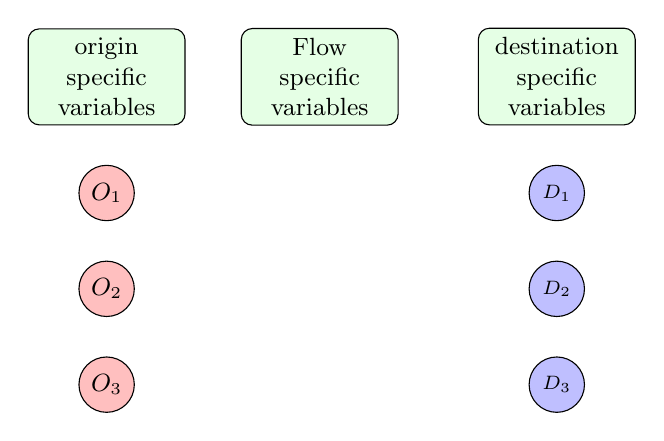
\begin{tikzpicture}[
             origin/.style={
         circle,
         draw=black,
         fill=red,
         fill opacity = 0.25,
         text opacity=1,
         inner sep=0pt,
         minimum size=20pt,
         font=\small},
       destination/.style={
         circle,
         draw=black,
         fill=blue,
         fill opacity = 0.25,
         text opacity=1,
         inner sep=0pt,
         minimum size=20pt,
         font=\scriptsize},
       var/.style = {rectangle, draw, fill=green!10, rounded corners, text centered, text width = 5em, minimum height = 2em, font= \small},
node distance=0.5cm and 5cm
      ]
      \node[origin] (O1) {$O_1$};
      \node[origin,below =  of O1] (O2) {$O_2$};
      \node[origin,below =  of O2] (O3) {$O_3$};

      \node[destination,right = of O1] (D1) {$D_1$};
      \node[destination,below =  of D1] (D2) {$D_2$};
      \node[destination,below =  of D2] (D3) {$D_3$};

      \node[var,  above = of O1] (O) {origin specific variables};
      \node[var,  above = of D1] (D) {destination specific variables};
      \node[var,  right = 0.7cm of O] (FD) {Flow specific variables};

\end{tikzpicture}         
		\caption{Variables that can affect flows $F_{ij}$ between origins $O_i$ and destinations $D_j$}
	\end{figure}
\end{frame}

  \section{Multilevel modeling}

  \begin{frame}{What is it?}
\begin{itemize}
\item Used in many disciplines, except economics (two-stage fixed effects regression)

    \item Simultenous modeling at various levels (e.g., cities, regions, flows, individuals)

    \item Many definitions:
    \begin{itemize}
    \item mixed effects 
    \item varying intercepts/parameter 
    \item shrinkage 
      \item partial pooling
          \end{itemize}
\end{itemize}

    
  \end{frame}

  \section{Data}


  \section{Results}

\begin{frame}[standout]
Thank you!
\end{frame}


\end{document}